\footnotesize
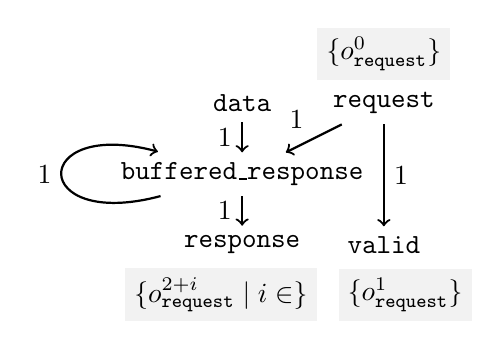
\begin{tikzpicture}[scale=.9,thick]
    \node (d) at (0, 0) {$\textpurple{\mathtt{data}}$};
    \node (rq) at (2, 0) {$\textpurple{\mathtt{request}}$};

    \node (br) at (0, -1) {$\mathtt{buffered\_response}$};
    \node (rp) at (0, -2) {$\mathtt{response}$};
    \node (v)  at (2, -2) {$\mathtt{valid}$};

    \draw[->] (d) -- node[left]{$1$} (br);
    \draw[->] (rq) -- node[above left]{$1$} (br);
    \draw[->] (br) edge[loop left] node{$1$} (br);
    \draw[->] (br) -- node[left]{$1$} (rp);
    \draw[->] (rq) -- node[right]{$1$} (v);


    \node[fill=gray!10] at (2, .7) {$\{o_{\mathtt{request}}^0\}$};
    \node[fill=gray!10] at (-.3, -2.7) {$\{o_{\mathtt{request}}^{2+i}\mid i\in\nats\}$};
    \node[fill=gray!10] at (2.3, -2.7) {$\{o_{\mathtt{request}}^1\}$};
\end{tikzpicture}
